\section{知识图谱}

\section{知识层次结构}

一元二次函数的知识不是平铺的一堆结论，而是有层次的。
下面这张图把知识分成六层：越靠下的层次越「具体好用」，
但都必须建立在上面几层的基础上。

\begin{figure}[htbp]
  \centering
  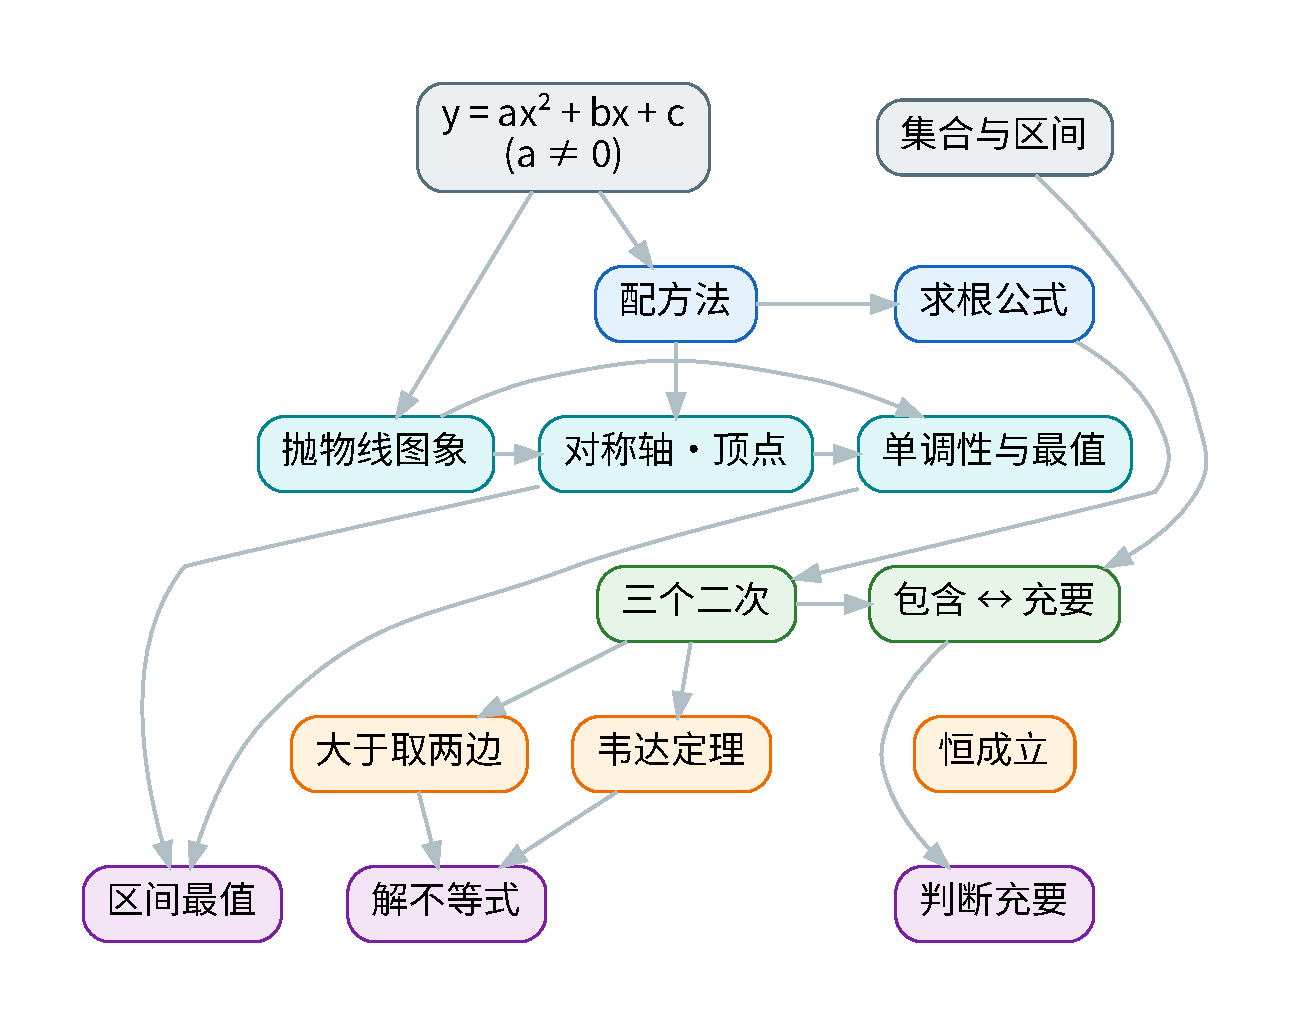
\includegraphics[width=\textwidth]{knowledge.pdf}
  \caption{一元二次函数的知识图谱}
\end{figure}

\section{六层结构说明}

\begin{enumerate}
  \item \key{事实层}：定义、符号、图象。这一层没有技巧，靠准确记忆。
  \item \key{操作层}：配方法、求根公式、解不等式的步骤。这一层靠动手练。
  \item \key{性质层}：开口、对称轴、顶点、单调性、最值。这一层靠看图总结。
  \item \key{关系层}：三个二次的统一、集合包含与充分必要条件的对应。这一层靠讲道理。
  \item \key{结论层}：韦达定理、口诀、恒成立条件。这一层靠会用。
  \item \key{策略层}：解题流程图。这一层靠照做。
\end{enumerate}

\section{学习建议}

基础较弱的同学，建议按下面的顺序过关：

\begin{enumerate}
  \item 先过\key{事实层}：能默写定义、说出符号含义；
  \item 再过\key{操作层}：配方、解方程各练熟；
  \item 然后过\key{性质层}：给一个解析式，能画出草图并说出性质；
  \item 最后再碰\key{结论层}：每条结论都要能说出它是从哪一层推出来的。
\end{enumerate}

\key{不要跳层。} 结论背得再熟，如果不知道它从哪来，换个条件就不会用。
